\section{DESENVOLVIMENTO}
Machine Learning, termo em inglês para aprendizagem de máquina, é a capacidade de computadores aprenderem a tomarem decisões sem que sejam previamente programados para isso. Esse aprendizado, assim como acontece boa parte do aprendizado humano, se dá através de erros e acertos, que são obtidos através de algoritmos matemáticos. Esses algoritmos matemáticos trabalham classificando variáveis, por exemplo, queremos que um computador seja capaz de distinguir um ser humano de um gavião. Para que o computador seja capaz de fazer essa distinção, fornecemos variáveis que serão utilizadas pelos algoritmos matemáticos para realizar as classificações. Nesse caso, fornecemos variáveis como, possui asas, capacidade de falar, capacidade de voar, capacidade de caminhar, possui bico, põe ovos, entre outras. Assim, após o algoritmo analisar os dados, o computador poderá distinguir com facilidade humanos de gaviões. 
É importante frisar que a qualidade da classificação se dá pela qualidade das variáveis, porque se utilizarmos variáveis como, possui olhos, respira, possui dedos ou ate mesmo se alimenta, nesse exemplo isso seria inútil para o algoritmo, uma vez que ambos os elementos comparados possuem essas características, assim, além de ser desprezível para o algoritmo, poderia até ser prejudicial para sua execução. 
O objetivo desse projeto é criar um sistema que ajude no tratamento de dados para predição de partidas de futebol, sendo assim, utilizamos durante a execução do projeto bases de dados disponíveis no site Football-Data \cite{FootballData2019}, e algumas das variáveis que utilizadas foram:
\begin{itemize}
	\item FTHG = Full Time Home Goals (Gols do time da casa no jogo)
	\item FTAG = Full Time Away Team Goals (Gols do time visitante no jogo)
	\item FTR = Full Time Result (Resultado do jogo)
	\item HTHG = Half Time Home Team Goals (Gols do time da casa no primeiro tempo)
	\item HTAG = Half Time Away Team Goals (Gols do time visitante no primeiro tempo)
	\item HTR = Half Time Result (Resultado do primeiro tempo)
	\item HS = Home Team Shots (Finalizações do time da casa)
	\item AS = Away Team Shots (Finalizações do time visitante)
	\item HST = Home Team Shots on Target (Finalizações certas do time da casa)
	\item AST = Away Team Shots on Target (Finalizações certas do time visitante)
	\item HHW = Home Team Hit Woodwork (Chutes na trave do time da casa)
	\item AHW = Away Team Hit Woodwork (Chutes na trave do time visitante)
	\item HC = Home Team Corners (Escanteios do time da casa)
	\item AC = Away Team Corners (escanteios do time visitante)
	\item HF = Home Team Fouls Committed (Faltas cometidas pelo time da casa)
	\item AF = Away Team Fouls Committed (Faltas cometidas pelo time visitante)
	\item HFKC = Home Team Free Kicks Conceded (Tiros de meta cedidos pelo time da casa)
	\item AFKC = Away Team Free Kicks Conceded (Tiros de meta cedidos pelo time visitante)
	\item HO = Home Team Offsides (Impedimentos do time da casa)
	\item AO = Away Team Offsides (Impedimentos do time visitante)
	\item HY = Home Team Yellow Cards (Cartões amarelos do time da casa)
	\item AY = Away Team Yellow Cards (Cartões amarelos do time visitante)
	\item HR = Home Team Red Cards (Cartões vermelhos do time da casa)
	\item AR = Away Team Red Cards (Cartões vermelhos do time visitante)
\end{itemize}
Essas variáveis apresentam importância significativa para os algoritmos, uma vez que podem determinar o andamento da partida e assim o resultado final.
A imagem a seguir apresenta os resultados da classificação com as seguintes variáveis: FTHG, FTAG, FTR, HTHG, HTAG, HTR, HS, AS, HST, AST, HF, AF, HC, AC, HY, AY, HR, AR.

\begin{figure}[htbp]
	\begin{center}
		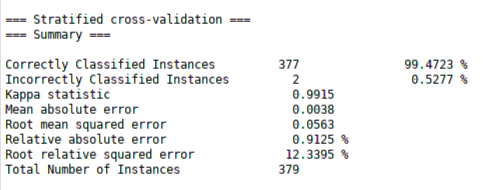
\includegraphics[width=.9\linewidth]{imagens/dados_completos.png}\\
	\end{center}
	\caption[Classificação com variáveis essenciais]{Classificação com variáveis essenciais}
	\label{fig:logo}
	%\legend{Fonte: Próprio Autor}
\end{figure}

E essa imagem apresenta os resultados com as seguintes variáveis: FTR, HTHG, HTAG, HS, AS, HST, AST, HF, AF, HC, AC, HY, AY, HR, AR.

\newpage

\begin{figure}[htbp]
	\begin{center}
		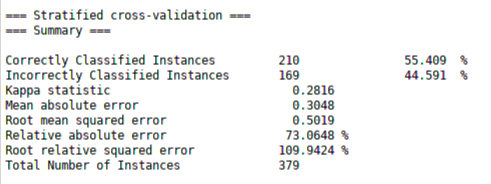
\includegraphics[width=.9\linewidth]{imagens/dados_incompletos.png}\\
	\end{center}
	\caption[Classificação com ausência de algumas variáveis essenciais]{Classificação com ausência de algumas variáveis essenciais}
	\label{fig:logo}
	%\legend{Fonte: Próprio Autor}
\end{figure}


Como é possível notar, a ausência das variáveis FTHG, FTAG, HTR fez com que o resultado final da classificação de instancias corretas caísse mais de 44 pontos percentuais, pois tais informações (gols do time da casa, gols do time visitante e resultado do primeiro tempo) são essenciais para definir o resultado final da partida.

Para auxiliar esse processo de escolha de variáveis, foi criado um sistema que funciona da seguinte maneira.

A página inicial é composta por dois elementos, sendo um botão do tipo input, que permite ao usuário a escolha da base de dados presente na máquina, e um outro botão do tipo submit que confirma o envio da base de dados para a pasta do projeto, para que seja utilizada nas demais telas.

A segunda página é composta por uma tabela que lista todos os dados da base de dados, permitindo a visualização completa desses dados. Nessa tela também estão presentes um elemento select multiple, que permite que o usuário escolha as colunas que irá usar para a construção de uma nova base de dados apenas com os dados selecionados pelo usuário.

A terceira página é responsável por listar os dado que foram selecionados na página anterior e gerar a base de dados limpa.
